\begin{name}
	{\tenchude}
	{ĐỀ TT LẦN 1 - SỞ THÁI NGUYÊN}
	{LỚP TOÁN THẦY PHÁT}
	{La confiance en soi est le premier secret du succès.}
\end{name}
\caulc
\Opensolutionfile{ans}[ans/ans\currfilebase]

\Opensolutionfile{ans}[ans/ans]
\begin{ex}%[1H8N7-3]%[Dự án C Đợt 3 NH25-26-Trường Sơn Hồng]%[Sở GD&ĐT Thái Nguyên]%[GV phản biện: Mui Đoan]
	Cho hình chóp $S.ABCD$ có $SA$ vuông góc với mặt phẳng $\left( ABCD \right)$, tứ giác $ABCD$ là hình vuông, $SA=3$ và $AB=1$. Thể tích của khối chóp $S.ABCD$ bằng
	\choice
	{$2$}
	{\True $1$}
	{$3$}
	{$9$}
	\loigiai{
		Diện tích hình vuông $ABCD$ là $S_{ABCD} = AB^2 = 1^2 = 1$. \\
		Chiều cao của khối chóp là $h = SA = 3$. \\
		Thể tích của khối chóp $S.ABCD$ là 
		$$V = \dfrac{1}{3} \cdot S_{ABCD} \cdot SA = \dfrac{1}{3} \cdot 1 \cdot 3 = 1.$$
	}
\end{ex}
%%---Câu 2---%%
\begin{ex}%[1H4N3-2]%[Dự án C Đợt 3 NH25-26-Trường Sơn Hồng]%[Sở GD&ĐT Thái Nguyên]%[GV phản biện: Mui Đoan]
	\immini[thm]{
		Cho hình hộp $ABCD.EFGH$ (tham khảo hình vẽ). Đường thẳng $GF$ song song với mặt phẳng nào sau đây?
		\choice
		{$\left( ACGE \right)$}
		{$\left( ABFE \right)$}
		{\True $\left( ABCD \right)$}
		{$\left( BDHF \right)$}
	}{
		\begin{tikzpicture}[line join = round,>=stealth, line cap = round, font = \small, scale = 0.7]
			\path  
			(0,0) coordinate (A) 
			(-1.5,-1) coordinate (B) 
			(2.5,-1) coordinate (C) 
			($(A)+(C)-(B)$) coordinate (D) 
			(-0.5,3.5) coordinate (E)
			($(B)+(E)-(A)$) coordinate (F) 
			($(C)+(E)-(A)$) coordinate (G) 
			($(D)+(E)-(A)$) coordinate (H) 
			; 
			\draw (F)--(G)--(H)--(E)--(F)--(B)--(C)--(G) (C)--(D)--(H);
			\draw[dashed] (B)--(A)--(E) (D)--(A);
			\foreach \x/\g in {E/90,F/130,G/110,H/90,A/140,B/-90,C/-90,D/-40} \fill (\x) circle (1.5pt) +(\g:3mm) node[scale=.8] {$\x$};
		\end{tikzpicture}
	}
	\loigiai{
		Trong hình hộp $ABCD.EFGH$, ta có $GF \parallel BC$ (vì $BCGF$ là hình bình hành). \\
		Mà đường thẳng $BC$ nằm trong mặt phẳng $\left( ABCD \right)$ và $GF$ không nằm trong mặt phẳng $\left( ABCD \right)$. \\
		Do đó, $GF \parallel \left( ABCD \right)$.
	}
\end{ex}
%%---Câu 3---%%
\begin{ex}%[1D6H4-2]%[Dự án C Đợt 3 NH25-26-Trường Sơn Hồng]%[Sở GD&ĐT Thái Nguyên]%[GV phản biện: Mui Đoan]
	Nghiệm của phương trình $\log_2 \left( x-1 \right)=3$ là
	\choice
	{\True $x=9$}
	{$x=4$}
	{$x=7$}
	{$x=10$}
	\loigiai{
		Điều kiện $x-1 > 0 \Leftrightarrow x > 1$.\\
		Phương trình đã cho tương đương với
		$$x-1 = 2^3 \Leftrightarrow x-1 = 8 \Leftrightarrow x = 9~\text{(thỏa mãn)}.$$
		Vậy nghiệm của phương trình là $x=9$.
	}
\end{ex}
%%---Câu 4---%%
\begin{ex}%[2D1N1-2]%[Dự án C Đợt 3 NH25-26-Trường Sơn Hồng]%[Sở GD&ĐT Thái Nguyên]%[GV phản biện: Mui Đoan]
	\immini[thm]{
		Cho hàm số đa thức bậc bốn $y = f(x)$ có đồ thị như hình vẽ. Hàm số đã cho đồng biến trên khoảng nào dưới đây?
		\choice
		{$\left( -1; 0 \right)$}
		{\True $\left( -\infty; -1 \right)$}
		{$\left( -\infty; 1 \right)$}
		{$\left( -1; +\infty \right)$}
	}{
		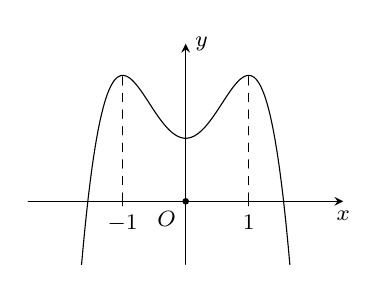
\begin{tikzpicture}[scale=0.8,line cap=round,line join=round,>=stealth,x=1.0cm,y=1.0cm]
			\draw[->,color=black] (-2.5,0.) -- (2.5,0.) node[below] {\footnotesize $x$};
			\foreach \x in {-1,1}
			\draw[shift={(\x,0)},color=black] (0pt,2pt) -- (0pt,-2pt) node[below] {\footnotesize $\x$};
			\draw[->,color=black] (0.,-1) -- (0.,2.5) node[right] {\footnotesize $y$};
			\draw[color=black] (0,0) node[below left] {\footnotesize $O$};
			\clip(-2.5,-1) rectangle (2.5,2.5);
			\draw[smooth,samples=100,domain=-2.5:2.5] plot(\x,{-(\x)^4+2*(\x)^2+1});
			\draw[dashed] (-1,0)--(-1,2) (1,0)--(1,2);
			\fill (0cm,0cm) circle (1.5pt); 
		\end{tikzpicture}
	}
	\loigiai{
		Dựa vào đồ thị hàm số, ta xác định các khoảng đơn điệu của hàm số như sau
		\begin{itemize}
			\item Đồ thị hàm số đi lên từ trái sang phải trên các khoảng $\left( -\infty; -1 \right)$ và $\left( 0; 1 \right)$, do đó hàm số đồng biến trên các khoảng này.
			\item Đồ thị hàm số đi xuống từ trái sang phải trên các khoảng $\left( -1; 0 \right)$ và $\left( 1; +\infty \right)$, do đó hàm số nghịch biến trên các khoảng này.
		\end{itemize}
		Trong các phương án đã cho, chỉ có khoảng $\left( -\infty; -1 \right)$ là khoảng đồng biến của hàm số.
	}
\end{ex}
%%---Câu 5---%%
\begin{ex}%[2D1N4-1]%[Dự án C Đợt 3 NH25-26-Trường Sơn Hồng]%[Sở GD&ĐT Thái Nguyên]%[GV phản biện: Mui Đoan]
	Tiệm cận ngang của đồ thị hàm số $y = \dfrac{2x - 5}{x + 2}$ là đường thẳng có phương trình
	\choice
	{$y = -2$}
	{$y = \dfrac{5}{2}$}
	{$y = \dfrac{2}{5}$}
	{\True $y = 2$}
	\loigiai{
		Tiệm cận ngang của đồ thị hàm số $y = \dfrac{ax+b}{cx+d}$ ($c \neq 0, ad-bc \neq 0$) là đường thẳng $y = \dfrac{a}{c}$. \\
		Với hàm số $y = \dfrac{2x - 5}{x + 2}$, ta có $a = 2, c = 1$. \\
		Vậy tiệm cận ngang của đồ thị hàm số là đường thẳng $y = \dfrac{2}{1} = 2$.
	}
\end{ex}
%%---Câu 6---%%
\begin{ex}%[2D4N1-4]%[Dự án C Đợt 3 NH25-26-Trường Sơn Hồng]%[Sở GD&ĐT Thái Nguyên]%[GV phản biện: Mui Đoan]
	Nguyên hàm của hàm số $f(x) = 2^x + x$ là
	\choice
	{$\dfrac{2^x}{\ln 2} + x^2 + C$}
	{\True $\dfrac{2^x}{\ln 2} + \dfrac{x^2}{2} + C$}
	{$2^x + \dfrac{x^2}{2} + C$}
	{$2^x + x^2 + C$}
	\loigiai{
		Ta có $\displaystyle \int f(x) \mathrm{\,d}x = \displaystyle \int \left( 2^x + x \right) \mathrm{\,d}x = \displaystyle \int 2^x \mathrm{\,d}x + \displaystyle \int x \mathrm{\,d}x = \dfrac{2^x}{\ln 2} + \dfrac{x^2}{2} + C$. \\
	}
\end{ex}
\begin{ex}%[2D1N5-1]%[Dự án C Đợt 3 NH25-26-Lê Hữu Kiệt]%[Sở GD&ĐT Thái Nguyên]%[GV phản biện: Mui Đoan]
	\immini
	{Đồ thị của hàm số nào dưới đây có dạng như đường cong trong hình vẽ?
		\choice[1]
		{$y = \dfrac{2x-1}{x+2}$}
		{\True $y = x^3 - 3x + 1$}
		{$y = -x^3 + 3x + 1$}
		{$y = \dfrac{x^2-1}{2x-1}$}
	}
	{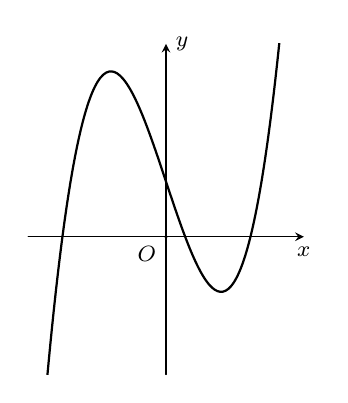
\begin{tikzpicture}[font=\footnotesize, line join=round, line cap=round, >=stealth, scale=0.7]
			\path (0,0) coordinate (O) (-2.5,0) coordinate (Xmin) (2.5,0) coordinate (Xmax) (0,-2.5) coordinate (Ymin) (0,3.5) coordinate (Ymax);
			\draw[->] (Xmin) -- (Xmax) node[below] {$x$};
			\draw[->] (Ymin) -- (Ymax) node[right] {$y$};
			\draw (O) node[below left] {$O$};
			\clip (-2.5,-2.5) rectangle (2.5,3.5);
			\draw[thick,smooth,samples=100,domain=-2.5:2.5] plot(\x,{(\x)^3-3*(\x)+1});
			\fill (O) circle (1pt);
	\end{tikzpicture}}
	\loigiai{
		Đường cong trong hình vẽ là đồ thị của hàm số bậc ba $y = ax^3 + bx^2 + cx + d$ với hệ số $a > 0$.\\
		Suy ra hàm số $y = x^3 - 3x + 1$ có đồ thị như hình đã cho.
	}
\end{ex}

% Câu TN 8
\begin{ex}%[2H2N2-2]%[Dự án C Đợt 3 NH25-26-Lê Hữu Kiệt]%[Sở GD&ĐT Thái Nguyên]%[GV phản biện: Mui Đoan]
	Trong không gian $Oxyz$, hình chiếu vuông góc của điểm $M(2;1;-1)$ trên mặt phẳng $(Oxz)$ có tọa độ là
	\choice
	{$(0;1;0)$}
	{$(2;1;0)$}
	{$(0;1;-1)$}
	{\True $(2;0;-1)$}
	\loigiai{
		Hình chiếu vuông góc của điểm $M(2;1;-1)$ trên $(Oxz)$ là điểm có tọa độ $(2;0;-1)$.
	}
\end{ex}

% Câu TN 9
\begin{ex}%[1D2N2-2]%[Dự án C Đợt 3 NH25-26-Lê Hữu Kiệt]%[Sở GD&ĐT Thái Nguyên]%[GV phản biện: Mui Đoan]
	Cho cấp số cộng $(u_n)$ có $u_1 = 2$ và $u_4 = 11$. Công sai của cấp số cộng đã cho bằng
	\choice
	{$1$}
	{$2$}
	{$4$}
	{\True $3$}
	\loigiai{
		Ta có $u_4 = u_1 + 3d \Leftrightarrow 11 = 2 + 3d \Leftrightarrow 3d = 9 \Leftrightarrow d = 3$.\\
		Vậy công sai của cấp số cộng bằng $3$.
	}
\end{ex}

% Câu TN 10
\begin{ex}%[2H2N2-3]%[Dự án C Đợt 3 NH25-26-Lê Hữu Kiệt]%[Sở GD&ĐT Thái Nguyên]%[GV phản biện: Mui Đoan]
	Trong không gian $Oxyz$, cho vectơ $\vec{a}=(2;-1;3)$, $\vec{b}=(1;3;-2)$. Tọa độ của vectơ $\vec{c} = \vec{a} - 2\vec{b}$ là
	\choice
	{\True $(0;-7;7)$}
	{$(4;-7;7)$}
	{$(0;7;7)$}
	{$(0;-7;-7)$}
	\loigiai{
		Ta có $2\vec{b} = (2;6;-4)$.\\
		Khi đó $\vec{c} = \vec{a} - 2\vec{b} = (2-2; -1-6; 3-(-4)) = (0;-7;7)$.
	}
\end{ex}

% Câu TN 11
\begin{ex}%[2D3H1-3]%[Dự án C Đợt 3 NH25-26-Lê Hữu Kiệt]%[Sở GD&ĐT Thái Nguyên]%[GV phản biện: Mui Đoan]
	Mỗi ngày bác An đều đi bộ để rèn luyện sức khỏe. Quãng đường đi bộ mỗi ngày của bác An trong $20$ ngày được thống kê ở bảng sau
	\begin{center}
		\begin{tabular}{|l|c|c|c|c|c|}
			\hline
			Quãng đường (km) & $[2{,}7;3{,}0)$ & $[3{,}0;3{,}3)$ & $[3{,}3;3{,}6)$ & $[3{,}6;3{,}9)$ & $[3{,}9;4{,}2)$ \\ \hline
			Số ngày & $3$ & $6$ & $5$ & $4$ & $2$ \\ \hline
		\end{tabular}
	\end{center}
	Khoảng tứ phân vị của mẫu số liệu ghép nhóm trên bằng
	\choice
	{$0{,}5$}
	{$0{,}9$}
	{\True $0{,}575$}
	{$0{,}975$}
	\loigiai{
		Tổng số ngày là $n=20$.
		\begin{itemize}
			\item Ta có $\dfrac{n}{4} = 5$. Nhóm chứa $Q_1$ là nhóm $[3{,}0;3{,}3)$. Khi đó
			$$Q_1 = 3{,}0 + \dfrac{5-3}{6} \cdot (3{,}3 - 3{,}0) = 3{,}1.$$
			\item Ta có $\dfrac{3n}{4} = 15$. Nhóm chứa $Q_3$ là nhóm $[3{,}6;3{,}9)$. Khi đó
			$$Q_3 = 3{,}6 + \dfrac{15-14}{4} \cdot (3{,}9 - 3{,}6) = 3{,}675.$$
		\end{itemize}
		Khoảng tứ phân vị là $\Delta_Q = Q_3 - Q_1 = 3{,}675 - 3{,}1 = 0{,}575$.
	}
\end{ex}

% Câu TN 12
\begin{ex}%[2D1N2-2]%[Dự án C Đợt 3 NH25-26-Lê Hữu Kiệt]%[Sở GD&ĐT Thái Nguyên]%[GV phản biện: Mui Đoan]
	Cho hàm số $f(x)$ có bảng biến thiên như hình vẽ. Giá trị cực tiểu của hàm số đã cho là
	\begin{center}
		
\begin{tikzpicture}[font=\footnotesize, line join=round, line cap=round, >=stealth, scale=1]
			\tkzTabInit[nocadre=false, lgt=1.2, espcl=2.5, deltacl=0.5]
			{$x$/0.6, $f'(x)$/0.6, $f(x)$/2}
			{$-\infty$, $-1$, $0$, $1$, $+\infty$}
			\tkzTabLine{ , +, 0, -, 0, +, 0, -, }
			\tkzTabVar{ -/ $-\infty$, +/ $2$, -/ $1$, +/ $2$, -/ $-\infty$ }
		\end{tikzpicture}
	\end{center}
	\choice
	{\True $y=1$}
	{$y=0$}
	{$y=-1$}
	{$y=2$}
	\loigiai{
		Dựa vào bảng biến thiên, ta thấy hàm số đạt cực tiểu tại $x=0$.\\
		Giá trị cực tiểu của hàm số là $y_{\text{CT}} = f(0) = 1$.
	}
\end{ex}

\TNTF

\begin{ex}%[Đề thi thử môn Toán Sở Thái Nguyên năm học 2025-2026]%[GVSB Trần Xuân Hòa - GV phản biện: Mui Đoan]%[2H2V2-4]
	Trong không gian gian với hệ tọa độ $Oxyz$, cho hình thang $ABCD$ vuông tại $A$ và $B$. Biết $A(1;2;1), B(2;0;-1), C(6;1;0)$ và diện tích hình thang $ABCD$ bằng $6\sqrt{2}$.
	\choiceTF
	{\True $\cos \left(\vec{AB},\vec{AC}\right) = \dfrac{\sqrt{3}}{3}$}
	{Tọa độ điểm $D$ là $(a;b;c)$. Khi đó $a+b+c = \dfrac{22}{3}$}
	{\True Gọi điểm $M(x_M;y_M;z_M)$ nằm trên mặt phẳng $(Oxy)$ thỏa mãn $MA^2 + 2MB^2 + 3MC^2$ đạt giá trị nhỏ nhất. Khi đó $x_M < 4$}
	{\True $\overrightarrow{AB}\cdot\overrightarrow{AC}=9$}
	\loigiai{Ta có $\overrightarrow{AB}=(1; -2; -2)$, $\overrightarrow{AC}=(5; -1; -1)$.
		\begin{center}
			\begin{tikzpicture}[scale=1, font=\footnotesize,line join=round, line cap=round, >=stealth]
				\path 
				(0,0) coordinate (A)
				++(-90:2) coordinate (B)
				++(0:4) coordinate (C)
				(2,0) coordinate (D)
				;
				\draw(A)--(B)--(C)--(D)--cycle;
				\pic[draw,angle eccentricity=1.8,angle radius=2mm]{right angle=B--A--D}
				pic[draw,angle eccentricity=1.8,angle radius=2mm]{right angle=C--B--A};
				\foreach \i/\g in {A/90,D/90,C/-90,B/-90}
				\fill[black] (\i) circle(1pt)+(\g:4mm)node[scale=1]{$\i$};
			\end{tikzpicture}
		\end{center}
		\begin{itemchoice}
			\itemch Vì 
			\begin{eqnarray*}
				\cos \left(\vec{AB},\vec{AC}\right)&=&\dfrac{\overrightarrow{AB}\cdot \overrightarrow{AC}}{|\overrightarrow{AB}|\cdot |\overrightarrow{AC}|}\\
				&=&\dfrac{1\cdot 5+(-2)\cdot (-1)+(-2)\cdot (-1)}{\sqrt{9}\cdot \sqrt{27}}\\
				&=&\dfrac{\sqrt{3}}{3}.
			\end{eqnarray*}
			
			\itemch Ta có $\overrightarrow{BC}=(4;1;1)$.\\
			Vì $\overrightarrow{AD}$ cùng hướng với $\overrightarrow{BC}$ nên $\overrightarrow{AD}=t\overrightarrow{BC}$, $t>0$.\\
			Ta có $BC=\sqrt{18}=3\sqrt{2}$, $AD=t\sqrt{18}=3t\sqrt{2}$.\\		
			Diện tích hình thang là
			\begin{eqnarray*}
				&&S=\dfrac{1}{2}(AD+BC)\cdot AB\\
				&\Leftrightarrow&6\sqrt{2}=\dfrac{1}{2}(3\sqrt{2}t+3\sqrt{2})\cdot 3\\
				&\Leftrightarrow&t=\dfrac{1}{3}.
			\end{eqnarray*}
			Do đó $\overrightarrow{AD}=\dfrac{1}{3}\overrightarrow{BC}$. Suy ra $D\left(\dfrac{7}{3};\dfrac{7}{3};\dfrac{4}{3}\right)$.\\
			Vậy $a+b+c=\dfrac{7}{3}+\dfrac{7}{3}+\dfrac{4}{3}=\dfrac{18}{3}=6$.
			\itemch Vì $M\in (Oxy)$ nên $M(a; b; 0)$.\\
			Ta có $\overrightarrow{MA}=(1-a; 2-b; 1)$, $\overrightarrow{MB}=(2-a; -b; -1)$, $\overrightarrow{MC}=(6-a; 1-b; 0)$.\\
			Xét
			\begin{eqnarray*}
				F&=&MA^2+2MB^2+3MC^2\\
				&=&\left[(1-a)^2+(2-b)^2+1\right]+2\left[(2-a)^2+(-b)^2+(-1)^2\right]+3\left[(6-a)^2+(1-b)^2\right]\\
				&=&6a^2-46a+6b^2-10b+123\\
				&=&6\left(a-\dfrac{23}{6}\right)^2+6\left(b-\dfrac{5}{6}\right)^2+\dfrac{92}{3}\\
				&\ge &\dfrac{92}{3}.
			\end{eqnarray*}
			Dấu \lq\lq = \rq\rq\, xảy ra khi và chỉ khi $a=\dfrac{23}{6}$ và $b=\dfrac{5}{6}$.\\
			Khi đó $F$ đạt giá trị nhỏ nhất khi $M\left(\dfrac{23}{6};\dfrac{5}{6};0\right)$.\\
			Do đó $x_M=\dfrac{23}{6}<4$.		
			\itemch Vì đã tính được  $\overrightarrow{AB}\cdot\overrightarrow{AC}=9$.
		\end{itemchoice}
	}
\end{ex}
\begin{ex}%[Đề thi thử môn Toán Sở Thái Nguyên năm học 2025-2026]%[GVSB Trần Xuân Hòa - GV phản biện: Mui Đoan]%[1D1H4-8]
	Trong hình vẽ sau đây, khi kéo ra khỏi vị trí cân bằng ở điểm $O$ và buông tay, lực đàn hồi của lò xo khiến vật $A$ gắn ở đầu của lò xo dao động quanh $O$. Tọa độ $s$ (centimét) của $A$ trên trục $Ox$ vào thời điểm $t$ (giây) sau khi buông tay được xác định bởi công thức $s = 10\sin\left(10t - \dfrac{\pi}{2}\right)$.
	\begin{center}
		\begin{tikzpicture}[>=stealth, line cap=round]
			
			% Mặt đất (gạch chéo)
			\fill[pattern=north east lines,line width=1mm] (-0.5,-0.6) rectangle (10,-1);
			
			% Tường bên trái
			\fill[pattern=north east lines,line width=.1mm] (-0.5,0.8) rectangle (0,-1);
			
			% Lò xo
			\draw[thick,decorate,decoration={coil,aspect=0.5,segment length=4pt,amplitude=4pt}]
			(0,0) -- (5,0);
			
			% Vật A
			\draw[thick,rounded corners=4pt,fill=red!10] (5,0.6) rectangle (7,-0.6);
			\node at (6,0.9) {A};
			
			% Điểm S (trong vật)
			\fill (6,0) circle (2pt);
			\node[below] at (6,0) {$S$};
			
			% Trục Ox
			\draw[->] (0,0) -- (9,0) node[right] {$x$};
			
			% Gốc O
			\fill (7.8,0) circle (2pt);
			\node[below] at (7.8,0) {$O$};
			
		\end{tikzpicture}
	\end{center}
	\choiceTF
	{Giá trị nhỏ nhất của hàm số $s = 10\sin\left(10t - \dfrac{\pi}{2}\right)$ bằng $-1$}
	{Thời điểm đầu tiên tọa độ của vật $A$ trên trục bằng $5$ là $t = \dfrac{2\pi}{15}$ (giây)}
	{\True Tập xác định của hàm số $s = 10\sin\left(10t - \dfrac{\pi}{2}\right)$ là $\mathbb{R}$}
	{\True Trong $3$ giây đầu tiên vật đi qua vị trí cân bằng $10$ lần}
	\loigiai{
		\begin{itemchoice}
			\itemch Vì $\sin \left(10t - \dfrac{\pi}{2}\right)\ge -1$ nên $s\ge -10$.\\
			Do đó giá trị nhỏ nhất của $s$ bằng $-10$.
			\itemch Xét phương trình
			\begin{eqnarray*}
				&&10\sin\left(10t-\dfrac{\pi}{2}\right)=5\\
				&\Leftrightarrow&\sin\left(10t-\dfrac{\pi}{2}\right)=\dfrac{1}{2}\\
				&\Leftrightarrow&\hoac{&10t-\dfrac{\pi}{2}=\dfrac{\pi}{6}+2k\pi\\& 10t-\dfrac{\pi}{2}=\dfrac{5\pi}{6}+2k\pi}\\
				&\Leftrightarrow&\hoac{&t= \dfrac{\pi}{15}+\dfrac{k\pi}{5}\\&t=\dfrac{2\pi}{15}+\dfrac{k\pi}{5}.}
			\end{eqnarray*}
			Thời điểm dương nhỏ nhất là $t=\dfrac{\pi}{15}$ ứng với $k=0$.
			\itemch Hàm số lượng giác xác định với mọi $t\in\mathbb{R}$.		
			\itemch Vật qua vị trí cân bằng khi 
			\begin{eqnarray*}
				&&s=0\\
				&\Leftrightarrow&\sin\left(10t - \dfrac{\pi}{2}\right) =0\\
				&\Leftrightarrow&\cos(10t)=0\\
				&\Leftrightarrow&10t=\dfrac{\pi}{2}+k\pi\\
				&\Leftrightarrow&t=\dfrac{\pi}{20}+\dfrac{k\pi}{10}.
			\end{eqnarray*}
			Xét 
			\begin{eqnarray*}
				&&0\le \dfrac{\pi}{20}+\dfrac{k\pi}{10}\le 3\\
				&\Leftrightarrow&-\dfrac{1}{2}\le k\le \dfrac{30}{\pi}-\dfrac{1}{2}\approx 9{,}05.
			\end{eqnarray*}
			Nên $k\in \{0; 1; 2;\ldots ; 9\}$.\\
			Số lần vật đi qua vị trí cân bằng trong $3$ giây đầu là $10$.
		\end{itemchoice}
	}
\end{ex}
\begin{ex}%[Đề thi thử môn Toán tỉnh Thái Nguyên năm học 2025-2026]%[Vũ Hồng Toàn - GV Mui Doan]%[2D4V1-6]
	Cây cà chua khi trồng có chiều cao $5$\,cm. Tốc độ tăng chiều cao của cây cà chua sau khi trồng $t$ tuần được cho bởi hàm số $v(t) = -0{,}1t^3 + t^2$, đơn vị: centimét/tuần. Gọi $h(t)$ là độ cao của cây cà chua ở tuần thứ $t$, đơn vị: centimét.
	\choiceTF
	{Vào thời điểm cây cà chua đó phát triển nhanh nhất, chiều cao của cây cà chua nhỏ hơn $54$\,cm}
	{\True Cây cà chua đó có thể phát triển và cao hơn $88$\,cm}
	{\True Tốc độ tăng chiều cao của cây cà chua sau khi trồng được $2$ tuần là $3{,}2$\,centimét/tuần}
	{Giai đoạn tăng trưởng của cây cà chua đó kéo dài $8$ tuần}
	\loigiai{
		\begin{itemchoice}
			\itemch Xét $v(t) = -0{,}1t^3 + t^2\Rightarrow v'(t) = -0{,}3t^2 + 2t$.\\
			Cho $v'(t)=0\Leftrightarrow -0{,}3t^2 + 2t=0\Leftrightarrow\hoac{&t=0\\&t = \dfrac{20}{3}.}$\\
			Bảng biến thiên
			\begin{center}
				
\begin{tikzpicture}
					\tkzTabInit[nocadre=false, lgt=1.2, espcl=4, deltacl=0.5]
					{$t$/0.7,$v’(t)$/0.7, $v(t)$/2}
					{$0$,$\tfrac{20}{3}$,$+\infty$}
					\tkzTabLine{,+,0,-,}
					\tkzTabVar{-/$0$,+/$\dfrac{400}{27}$,-/$-\infty$}
				\end{tikzpicture}
			\end{center}
			Từ bảng biến thiên suy ra thời điểm cây phát triển nhanh nhất khi $t = \dfrac{20}{3}$\,tuần.\\
			Ta có
			\begin{align*}
				h(t)&=\displaystyle\int v(t)\mathrm{\,d}t\\
				&=\displaystyle\int \left(-0{,}1t^3 + t^2\right)\mathrm{d}t\\
				&=-\dfrac{1}{40}t^4+\dfrac{1}{3}t^3+C.
			\end{align*}
			Do cây cà chua khi trồng có chiều cao $5$\,cm nên $h(0)=5$.\\ Suy ra
			\begin{align*}
				-\dfrac{1}{40}\cdot 0^4+\dfrac{1}{3}\cdot 0^3+C=5\Rightarrow C=5.
			\end{align*}
			Khi đó $h(t)=-\dfrac{1}{40}t^4+\dfrac{1}{3}t^3+5$.\\
			Vậy $h\left(\dfrac{20}{3}\right) = -\dfrac{1}{40} \cdot \left(\dfrac{20}{3}\right)^4 + \dfrac{1}{3} \cdot \left(\dfrac{20}{3}\right)^3 + 5 \approx 54{,}38$\,(cm).
			\itemch Giai đoạn tăng trưởng kết thúc khi $v(t) = 0 \Leftrightarrow -0{,}1t^3 + t^2 = 0 \Leftrightarrow \hoac{&t=0\\&t=10.}$\\
			Chiều cao tối đa cây đạt được tại $t = 10$\,(tuần). Do đó
			\[ h(10) = -\dfrac{1}{40}\cdot 10^4 + \dfrac{1}{3}\cdot 10^3 + 5 \approx 88{,}33 \text{ (cm)}. \]
			\itemch Tốc độ tăng chiều cao của cây cà chua sau khi trồng được $2$ tuần là
			\[v(2) = -0{,}1\cdot 2^3 + 2^2 = 3{,}2 \text{ (cm/tuần)}.\]
			\itemch Cây tăng trưởng chiều cao khi
			\begin{eqnarray*}
				&&v(t) \ge 0\\
				&\Leftrightarrow&-0{,}1t^3 + t^2\ge 0\\
				&\Leftrightarrow& 0\le t\le 10.
			\end{eqnarray*}
			Vậy, giai đoạn tăng trưởng của cây cà chua kéo dài $10$ tuần kể từ khi trồng.
		\end{itemchoice}
	}
\end{ex}
%%%==============HetCau_3==============%%%

%%%==============Cau_4==============%%%
\begin{ex}%[Đề thi thử môn Toán tỉnh Thái Nguyên năm học 2025-2026]%[GV soạn: Vũ Hồng Toàn - GVPB: Mui Doan]%[2D1V3-1]
	Cho hàm số $y = f(x) = (x^2 - 5x + 7)\mathrm{e}^x$.
	\choiceTF
	{\True $f(0) = 7$}
	{Hàm số $y = f(x)$ nghịch biến trên khoảng $\left(-\infty; \dfrac{5}{2}\right)$}
	{Đạo hàm của hàm số đã cho là $f'(x) = (2x - 5)\mathrm{e}^x$}
	{\True Giá trị nhỏ nhất của hàm số $y = f(x)$ trên đoạn $[0;2]$ bằng $7$}
	\loigiai{
		Tập xác định $\mathscr{D}=\mathbb{R}$.\\
		Ta có
		\begin{eqnarray*}
			f(x) &=& (x^2 - 5x + 7)\mathrm{e}^x\\
			\Rightarrow f'(x)&=&(2x - 5)\mathrm{e}^x + (x^2 - 5x + 7)\mathrm{e}^x\\
			&=&(x^2 - 3x + 2)\mathrm{e}^x.
		\end{eqnarray*}
		\begin{itemchoice}
			\itemch Ta có $f(0) = (0^2 - 5 \cdot 0 + 7) \cdot \mathrm{e}^0 = 7 \cdot 1 = 7$.
			\itemch Cho $f'(x)=0\Leftrightarrow (x^2 - 3x + 2)\mathrm{e}^x\Leftrightarrow \hoac{&x=1\\&x=2.}$\\
			Bảng biến thiên
			\begin{center}
				
\begin{tikzpicture}
					\tkzTabInit[nocadre=false, lgt=1.2, espcl=3, deltacl=0.5]
					{$x$/0.7,$f’(x)$/0.7,$f(x)$/2}
					{$-\infty$,$1$,$2$,$+\infty$}
					\tkzTabLine{,+,0,-,0,+,}
					\tkzTabVar{-/$-\infty$,+/$3\mathrm{e}$,-/$\mathrm{e}^2$,+/$+\infty$}
				\end{tikzpicture}
			\end{center}
			Từ bảng biến thiên ta thấy, hàm số đã cho nghịch biến trên khoảng $(1;2)$.
			\itemch Ta có $f'(x)=(x^2 - 3x + 2)\mathrm{e}^x$.
			\itemch Ta có $f(0)=7$, $f(1)=3\mathrm{e}$, $f(2)=\mathrm{e}^2$.\\
			Vậy $\min\limits_{[0;2]}f(x)=f(0)=7$.
		\end{itemchoice}
	}
\end{ex}
%%%==============HetCau_4==============%%%

\TNSA
%%=======Câu 1=======%%
\begin{ex}%[0D8V1-2]%[Đề thi thử môn Toán SGD Thái Nguyên năm học 2025-2026]%[Đỗ Nam - GVPB: Mui Doan]
	Có bao nhiêu cách chọn sáu số từ chín số nguyên $1$, $2$, $\ldots$, $9$ và điền vào các ô của hình dưới đây (mỗi ô chỉ điền đúng một số) sao cho tổng các số ở mỗi cột (kể cả cột có một ô) bằng nhau?
	\begin{center}
		\begin{tikzpicture}[scale=0.8,rotate=90, line join=round, line cap=round]
			\draw (0,0) rectangle (1,1);
			\draw (1,0) rectangle (2,1);
			\draw (2,0) rectangle (3,1);
			\draw (0,1) rectangle (1,2);
			\draw (1,1) rectangle (2,2);
			\draw (0,2) rectangle (1,3);
		\end{tikzpicture}
	\end{center}
	\shortans{48}
	\loigiai{
		Gọi các số ở các cột như sau:
		\begin{itemize}
			\item Cột $1$ có $1$ ô chứa số $f$.
			\item Cột $2$ có $2$ ô chứa các số $d$, $e$.
			\item Cột $3$ có $3$ ô chứa các số $a$, $b$, $c$.
		\end{itemize}
		Theo bài toán, ta có tổng ở mỗi cột là $f=d+e=a+b+c=S$.\\
		Vì các số được chọn từ tập $\{1;2;\ldots;9\}$ và đôi một khác nhau nên ta có
		\begin{itemize}
			\item Vì cột $1$ chứa $1$ số $f$ nên $S=f$. Do đó $S\in\{1;2;\ldots;9\}$.
			\item Vì cột $3$ chứa $3$ số phân biệt nên tổng nhỏ nhất có thể là $1+2+3=6$. Do đó $S\geq 6$.
		\end{itemize}
		Từ đó, ta được $S\in\{6;7;8;9\}$.\\
		Xét các trường hợp của $S$ như sau:
		\begin{itemize}
			\item \textbf{TH1:} $S=6$.
			\begin{itemize}
				\item Cột $1$: $f=6$.
				\item Cột $2$: $d+e=6$ nên $\{d;e\}=\{1;5\}$ hoặc $\{2;4\}$.
				\item Cột $3$: $a+b+c=6$ nên $\{a;b;c\}=\{1;2;3\}$.
			\end{itemize}
			Vì cột $3$ và cột $2$ bị trùng các số $1$ và $2$ nên trường hợp này không xảy ra.
			\item \textbf{TH2:} $S=7$.
			\begin{itemize}
				\item Cột $1$: $f=7$.
				\item Cột $2$: $d+e=7$ nên $\{d;e\}=\{1;6\}$, $\{2;5\}$ hoặc $\{3;4\}$.
				\item Cột $3$: $a+b+c=7$ nên $\{a;b;c\}=\{1;2;4\}$.
			\end{itemize}
			Vì cột $3$ và cột $2$ bị trùng các số $1$, $2$ và $4$ nên trường hợp này không xảy ra.
			\item \textbf{TH3:} $S=8$.
			\begin{itemize}
				\item Cột $1$: $f=8$.
				\item Cột $2$: $d+e=8$ nên $\{d;e\}=\{1;7\}$, $\{2;6\}$ hoặc $\{3;5\}$.
				\item Cột $3$: $a+b+c=8$ nên $\{a;b;c\}=\{1;2;5\}$, $\{1;3;4\}$.
			\end{itemize}
			Ta thấy, cột $3$ chọn $\{a;b;c\}=\{1;3;4\}$ và cột $2$ chọn $\{d;e\}=\{2;6\}$ thỏa mãn yêu cầu bài toán và không bị trùng.
			\item \textbf{TH4:} $S=9$.
			\begin{itemize}
				\item Cột $1$: $f=9$.
				\item Cột $2$: $d+e=9$ nên $\{d;e\}=\{1;8\}$, $\{2;7\}$, $\{3;6\}$ hoặc $\{4;5\}$.
				\item Cột $3$: $a+b+c=9$ nên $\{a;b;c\}=\{1;2;6\}$, $\{1;3;5\}$ hoặc $\{2;3;4\}$.
			\end{itemize}
			Từ đó, ta thấy
			\begin{itemize}
				\item Nếu cột $3$ chọn $\{a;b;c\}=\{1;2;6\}$ và cột $2$ chọn $\{d;e\}=\{4;5\}$ thì không bị trùng và thỏa mãn yêu cầu bài toán.
				\item Nếu cột $3$ chọn $\{a;b;c\}=\{2;3;4\}$ và cột $2$ chọn $\{d;e\}=\{1;8\}$ thì vừa không bị trùng, vừa thỏa mãn yêu cầu bài toán.
				\item Nếu cột $3$ chọn $\{a;b;c\}=\{1;3;5\}$ và cột $2$ chọn $\{d;e\}=\{2;7\}$ thì vừa không bị trùng, vừa thỏa mãn yêu cầu bài toán.
			\end{itemize}
		\end{itemize}
		Khi đó, với mỗi bộ số tìm được, ta có số cách xếp vào ô là
		\begin{itemize}
			\item Số cách xếp cột $1$ là $1!=1$ cách.
			\item Số cách xếp cột $2$ là $2!=2$ cách.
			\item Số cách xếp cột $3$ là $3!=6$ cách.
		\end{itemize}
		Suy ra, số cách xếp cho mỗi bộ số thỏa mãn yêu cầu bài toán là $1\cdot2\cdot6=12$ cách.\\
		Mặt khác, ta có $4$ bộ thỏa mãn yêu cầu là $\{1;3;4;2;6;8\}$, $\{1;2;6;4;5;9\}$, $\{2;3;4;1;8;9\}$ và $\{1;3;5;2;7;9\}$.\\
		Vậy tổng số cách xếp là $12\cdot4=48$.
	}
\end{ex}
%%=======Câu 2=======%%
\begin{ex}%[1H8V6-2]%[Đề thi thử môn Toán SGD Thái Nguyên năm học 2025-2026]%[Đỗ Nam - GVPB: Mui Doan]
	Cho tứ diện $ABCD$ có $\widehat{BAC}=30^\circ$, $\widehat{CAD}=45^\circ$, $\widehat{DAB}=60^\circ$. Gọi $\alpha=[B,AD,C]$ thì giá trị của $\cos\alpha$ bằng bao nhiêu? (không làm tròn kết quả các phép tính trung gian, chỉ làm tròn kết quả cuối cùng đến hàng phần trăm)
	\shortans{0{,}84}
	\loigiai{
		\begin{center}
			\begin{tikzpicture}[font=\footnotesize,line join=round, line cap=round, >=stealth,scale=0.8] 
				\def\a{6}
				\def\b{3}
				\def\h{4}	
				\path (0,0) coordinate (B)
				(0:\a) coordinate (D)
				(-40:\b) coordinate (C)
				($(C)!0.5!(D)$)coordinate(I)
				($(B)!2/3!(I)$)coordinate(O)
				($(O)+(90:\h)$) coordinate (A)
				($(A)!(C)!(D)$)coordinate(H)
				($(C)!0.5!(A)$)coordinate(K)
				($(A)!(K)!(D)$)coordinate(M)
				;	
				\draw (B)--(C)--(D)-- (A)--(B)--(K)--(M) (A)--(C)--(H);
				\draw[dashed] (B)--(D) (M)--(B);
				\foreach \x/\y/\z in {C/H/A,K/M/A} \draw pic[draw,angle radius=2mm]
				{right angle= \x--\y--\z};
				\foreach \x/\y/\z in {B/M/K} \draw pic[draw,angle radius=5mm]
				{angle= \x--\y--\z};
				\foreach \x/\y/\z in {B/M/K} \draw pic[draw,angle radius=5.5mm]
				{angle= \x--\y--\z};
				\foreach \x/\pos in {A/90,B/180,C/-45,D/0,H/0,K/-45,M/45} \fill (\x) circle(1pt) node[{shift=(\pos:0.25)}]{$\x$}; 
			\end{tikzpicture}
		\end{center}
		Kẻ $BM\perp AD$ tại $M$, $CH\perp AD$ tại $H$.\\
		Kẻ $KM \parallel CH$.\\
		Ta có $\heva{&BM\perp AD\\&KM\perp AD\text{ (vì $CH\perp AD$)}.}$\\
		Suy ra $\alpha=[B,AD,C]=\widehat{BMK}$.\\
		Xét $\triangle ABM$ vuông tại $M$, ta có\\
		$BM=AB\cdot\sin60^{\circ}=\dfrac{\sqrt{3}}{2}\cdot AB$.\\
		$AM=AB\cdot\cos60^{\circ}=\dfrac{1}{2}\cdot AB$.\\
		Mà $\triangle AMK$ có $\widehat{KAM}=45^{\circ}$ và $\widehat{KMA}=90^{\circ}$.\\
		Suy ra $\triangle AMK$ vuông cân tại $M$ nên $AM=KM=\dfrac{1}{2}\cdot AB$.\\
		Xét $\triangle AMK$ vuông tại $M$, ta có $AK^2=AM^2+KM^2=2\cdot KM^2$.\\
		Suy ra $AK=\sqrt{2}\cdot KM=\sqrt{2}\cdot\dfrac{1}{2}\cdot AB=\dfrac{AB\sqrt{2}}{2}$.\\
		Xét $\triangle ABK$, theo định lí Côsin ta có
		\begin{align*}
			BK&=\sqrt{AB^2+AK^2-2\cdot AB\cdot AK\cos\widehat{BAK}}\\
			&=\sqrt{AB^2+\dfrac{AB^2}{2}-2\cdot AB\cdot\dfrac{AB\sqrt{2}}{2}\cdot\cos30^{\circ}}\\
			&=AB\cdot\sqrt{\dfrac{3-\sqrt{6}}{2}}. 
		\end{align*}
		Theo định lí Côsin, ta có 
		\[\cos\widehat{BMK}=\dfrac{BM^2+KM^2-BK^2}{2BM\cdot KM}=\dfrac{\left(\dfrac{\sqrt{3}}{2}\cdot AB\right)^2+\left(\dfrac{1}{2}\cdot AB\right)^2-\left(AB\cdot\sqrt{\dfrac{3-\sqrt{6}}{2}}\right)^2}{2\cdot\dfrac{\sqrt{3}}{2}\cdot AB\cdot\dfrac{1}{2}\cdot AB}\approx0{,}84.\]
	}
\end{ex}
%3
\begin{ex}%[2D4V2-6]%[Dự án đề kiểm tra TT-SGD-ThaiNguyen-NH25-26 - Hứa Chí Ninh- GVPB: Mui Doan]
	Đối với ngành nuôi trồng thủy sản, việc kiểm soát lượng thuốc tồn dư trong nước là một nhiệm vụ quan trọng nhằm đáp ứng các tiêu chuẩn an toàn về môi trường. Khi nghiên cứu một loại thuốc trị bệnh trong nuôi trồng thủy sản, người ta sử dụng thuốc đó một lần và theo dõi nồng độ thuốc tồn dư trong nước kể từ lúc sử dụng thuốc. Kết quả cho thấy nồng độ thuốc $y(t)$ (đơn vị: mg/lít) tồn dư trong nước tại thời điểm $t$ ngày kể từ lúc sử dụng thuốc, thỏa mãn $y(t) = \mathrm{e}^{g(t)}$ và $y'(t) = k \cdot y(t)$ với $t \geq 0$, trong đó $k$ là hằng số khác không. Đo nồng độ thuốc tồn dư trong nước tại các thời điểm $t=6$ ngày, $t=12$ ngày nhận được kết quả lần lượt là $2$ mg/lít, $1$ mg/lít. Nồng độ thuốc tồn dư trong nước tại thời điểm $30$ ngày bằng bao nhiêu mg/lít (Kết quả làm tròn đến hàng phần trăm)?
	\shortans{$0{,}13$} 
	\loigiai{
		Từ giả thiết, ta có
		\begin{eqnarray*}
			y'(t) &=& k \cdot y(t)\\
			\Rightarrow \dfrac{y'(t)}{y(t)} &=& k\\
			\Rightarrow \ln |y(t)| &=& kt + C.
		\end{eqnarray*}
		Vì $y(t) = \mathrm{e}^{g(t)} > 0$ nên $y(t) = \mathrm{e}^{kt+C} = A \cdot \mathrm{e}^{kt}$ (với $A = \mathrm{e}^C$).
		\begin{itemize}
			\item Tại $t=6$ thì $y(6) = A \cdot \mathrm{e}^{6k} = 2$.
			\item Tại $t=12$ thì $y(12) = A \cdot \mathrm{e}^{12k} = 1$.
		\end{itemize}
		Suy ra $$\dfrac{y(12)}{y(6)} = \dfrac{\mathrm{e}^{12k}}{\mathrm{e}^{6k}} = \dfrac{1}{2} \Rightarrow \mathrm{e}^{6k} = \dfrac{1}{2} \Rightarrow \mathrm{e}^k = \left(\dfrac{1}{2}\right)^{\frac{1}{6}}.$$
		Thay vào $y(6)$, ta được $$A \cdot \dfrac{1}{2} = 2 \Rightarrow A = 4.$$
		Vậy $y(t) = 4 \cdot \left(\dfrac{1}{2}\right)^{\frac{t}{6}}.$
		Khi $t=30$, ta được $y(30) = 4 \cdot \left(\dfrac{1}{2}\right)^{\frac{30}{6}} = 4 \cdot \left(\dfrac{1}{2}\right)^5 = \dfrac{4}{32} = 0{,}125 \approx 0{,}13$.
	}
\end{ex}

\begin{ex}%[2H5V2-6]%[Dự án đề kiểm tra TT-SGD-ThaiNguyen-NH25-26 - Hứa Chí Ninh - GVPB: Mui Doan]
	Cho hình hộp chữ nhật $ABCD.EFGH$ với $AB=6$, $AD=8$ và $DH=10$. Gọi điểm $M$ là trung điểm của đoạn thẳng $AF$ và điểm $I$ thuộc mặt phẳng $(ABCD)$. Khi $IM+IG$ nhỏ nhất thì điểm $I$ cách hai đường thẳng $BA$ và $BC$ tương ứng bằng $a$ và $b$. Giá trị của biểu thức $P=3a+6b$ bằng bao nhiêu?
	\shortans{$20$}
	\loigiai{
		\begin{center}
			\begin{tikzpicture}[>=stealth, line join=round, line cap=round]
				% 1. Định nghĩa tọa độ các điểm theo đúng phối cảnh hình bạn gửi
				\coordinate (A) at (0,0,0);
				\coordinate (B) at (-1.2,-1.5,0); % Trục x chéo xuống trái
				\coordinate (D) at (4,0,0);      % Trục y nằm ngang
				\coordinate (C) at ($(B)+(D)-(A)$);
				
				\def\h{3} % Chiều cao khối hộp
				\coordinate (E) at (0,\h);
				\coordinate (F) at ($(B)+(0,\h)$);
				\coordinate (F') at ($(B)+(B)-(F)$);
				\coordinate (G) at ($(C)+(0,\h)$);
				\coordinate (M) at ($(A)!0.5!(F)$);
				\coordinate (M') at ($(A)!0.5!(F')$);
				\coordinate (H) at ($(D)+(0,\h)$);
				\coordinate (I) at ($(M')!0.3!(G)$);	
				\coordinate (J) at ($(M')!0.2!(G)$);	
				\coordinate (K) at ($(M')!0.25!(M)$);	
				
				\draw[dashed] (D)--(A) -- (B);
				\draw[dashed] (F)-- (A) -- (E);
				\draw[dashed] (I)--(M) -- (M')--(G);
				
				\draw[thick] (B) -- (C) -- (D);
				\draw[thick] (B) -- (F) -- (G) -- (C) -- cycle;
				\draw[thick] (G) -- (H) -- (D);
				\draw[thick] (E) -- (F);
				\draw[thick] (E) -- (H);
				\draw[thick] (J) -- (M')--(K);
				
				% 4. Vẽ hệ trục tọa độ
				\draw[->] (B) -- ++(-1,-1) node[below left] {$x$};
				\draw[->] (D) -- ++(1,0) node[below] {$y$};
				\draw[->] (E) -- ++(0,1) node[left] {$z$};
				
				
				\foreach \p/\pos in {A/above right, B/below, C/below, D/below, E/left, F/left, G/right, H/above,M/right,M'/right,I/right}
				\fill (\p) circle (1pt) node[\pos] {\small $\p$};
			\end{tikzpicture}
		\end{center}
		Chọn hệ trục tọa độ $Oxyz$ với $A(0;0;0)$, $B(6;0;0)$, $D(0;8;0)$, $E(0;0;10)$, khi đó $C(6;8;0)$, $F(6;0;10)$, $G(6;8;10)$.\\
		Vì $M$ là trung điểm $AF$ nên $M(3;0;5)$.\\
		Điểm $I$ thuộc mặt phẳng $(ABCD)$, mà mặt phẳng $(ABCD)$ chính là mặt phẳng $Oxy$ nên $I(x;y;0)$.\\
		Để $IM+IG$ nhỏ nhất, ta lấy điểm $M'$ đối xứng với $M$ qua mặt phẳng $(ABCD)$.\\
		Vì $M(3;0;5)$ và mặt phẳng đối xứng là $z=0$ nên $M'(3;0;-5)$.\\
		Khi đó $$IM+IG = IM'+IG \geq M'G.$$
		Dấu "$=$" xảy ra khi $I$ là giao điểm của $M'G$ và mặt phẳng $(ABCD)$.\\
		Ta có $\overrightarrow{M'G} = (3;8;15)$, suy ra
		$$M'G \colon \heva {&x = 3+3t \\ &y = 8t \\ &z = -5+15t.}$$
		Vì $I \in M'G$ nên $I(3+3t,8t,-5+15t)$.\\
		Lại có $I \in (ABCD)$ nên $-5+15t = 0 \Rightarrow t = \dfrac{1}{3}$. Do đó $I(4; \dfrac{8}{3}; 0)$.
		\begin{itemize}
			\item Khoảng cách từ $I$ đến $BA$ (trục $Ox$) là $a = \left| y_I \right| = \dfrac{8}{3}$.
			\item Khoảng cách từ $I$ đến $BC$ là $b = \left| 6 - x_I \right| = \left| 6 - 4 \right| = 2$.
		\end{itemize}
		Vậy $P = 3a + 6b = 3 \cdot \dfrac{8}{3} + 6 \cdot 2 = 8 + 12 = 20$.}
\end{ex}
%-----Câu 3
\begin{ex}%[0D2V2-3]%[Dự án đề TT THPTQG NH25-26-Dot 3- Nguyễn Tá- GVPB: Mui Doan]%[SGD Thái Nguyên]
	Trong một cuộc thi pha chế, mỗi đội chơi được sử dụng tối đa $24$ gam hương liệu, $9$ lít nước và $210$
	gam đường để pha chế nước ngọt loại I và nước ngọt loại II. Để pha chế $1$ lít nước ngọt loại I cần $10$ gam
	đường, $1$ lít nước và $4$ gam hương liệu. Để pha chế $1$ lít nước ngọt loại II cần $30$ gam đường, $1$ lít nước và $1$
	gam hương liệu. Mỗi lít nước ngọt loại I được $80$ điểm thưởng, mỗi lít nước ngọt loại II được $60$ điểm thưởng.
	Hỏi số điểm thưởng tối đa mà một đội trong cuộc thi có thể đạt được là bao nhiêu?
	\shortans{$640$}
	\loigiai{Gọi $x$ (lít) là thể tích nước ngọt loại $I$ được pha chế ($x\ge 0$).\\
		Gọi $y$ (lít) là thể tích nước ngọt loại $II$ được pha chế ($y\ge 0$).\\
		Do để pha chế nước $1$ lít ngọt loại $I$ cần $10$ gam đường và để pha chế $1$ lít nước ngọt loại $II$ cần $30$ gam đường nên 
		\begin{equation*}
			10x+30y \le 210.
		\end{equation*}
		Tương tự do để pha chế nước $1$ lít ngọt loại $I$ và $1$ lít ngọt loại $II$ đều cần $1$ lít nước nên 
		\begin{equation*}
			x+y \le 9.
		\end{equation*}
		Cuối cùng để pha chế nước $1$ lít ngọt loại $I$ cần $4$ gam hương liệu và để pha chế $1$ lít nước ngọt loại $II$ cần $1$ gam hương liệu nên 
		\begin{equation*}
			4x+y \le 24.
		\end{equation*}
		Số điểm thưởng có thể của mỗi đội là $F(x,y)=80x+60y$, với $x$, $y$ thỏa mãn hệ bất phương trình
		\begin{equation*}
			\heva{&10x+30y \le 210\\&x+y \le 9\\&4x+y \le 24\\&x,y \ge 0.}
		\end{equation*}
		Miền nghiệm của hệ bất phương trình là đa giác $OABCD$ được tô màu như hình vẽ
		dưới và có các đỉnh là
		$A(0;7)$,  $B(3;6)$,  $C(5;4)$, $D(6;0)$, $O(0;0)$.
		\begin{center}
			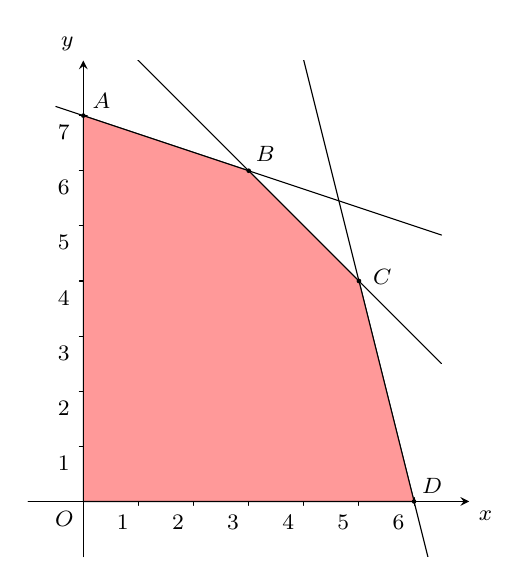
\begin{tikzpicture}[scale=0.7,font=\footnotesize,line join=round,line cap=round,>=stealth]
				% Trục Ox
				\draw[->] (-1,0) -- (7,0) node[below right] {$x$};
				% Trục Oy
				\draw[->] (0,-1) -- (0,8) node[above left] {$y$};
				% Gốc tọa độ
				\node[below left] at (0,0) {$O$};
				\clip(-1,-1) rectangle (7,8);
				\draw[smooth,samples=100,domain=-0.5:6.5] plot (\x, 7-\x/3);
				\draw[smooth,samples=100,domain=-0.5:6.5] plot (\x, 9-\x);
				\draw[smooth,samples=100,domain=-0.5:6.5] plot (\x, 24-4*\x);
				\foreach \y in {1,2,3,4,5,6,7} 
				\draw[shift={(0,\y)},color=black] (2pt,0pt) -- (-2pt,0pt) node[below left] { $\y$};
				\foreach \x in {1,2,3,4,5,6} 
				\draw[shift={(\x,0)},color=black] (0pt,2pt) -- (0pt,-2pt) node[below left] { $\x$};
				\path (0,7) coordinate (A)
				(3,6) coordinate (B)
				(5,4) coordinate (C)
				(6,0) coordinate (D)
				(0,0) coordinate (O)
				;
				\draw[fill=red!40] (A)--(B)--(C)--(D)--(O)--cycle;
				\foreach \p/\r in {A/40,B/45,C/10,D/40}
				\fill (\p) circle (1.2pt) node[shift={(\r:3mm)}]{$\p$};
			\end{tikzpicture}
		\end{center}
		Ta có
		\begin{equation*}
			\heva{&F(0,7)=80\cdot0+60\cdot7=420\\&F(3,6)=80\cdot3+60\cdot6=600\\&F(5,4)=80\cdot5+60\cdot4=640\\&F(6,0)=80\cdot6+60\cdot 0=480\\&F(0,0)=80\cdot0+60\cdot0=0.}
		\end{equation*}
		Do đó số điểm cao nhất là $F(5,4)=640$.
	}
\end{ex}
%-----Câu 4
\begin{ex}%[0D0V2-2]%[Dự án đề TT THPTQG NH25-26-Dot 3- Nguyễn Tá- GVPB: Mui Doan]%[SGD Thái Nguyên]
	Tung đồng thời hai con xúc xắc khác nhau đều cân đối và đồng chất ba lần. Bằng cách cộng số chấm xuất hiện trên hai con xúc xắc trong mỗi lần tung ta được một số ngẫu nhiên từ $2$ đến $12$. Gọi ba số này lần
	lượt là $a$, $b$ và $t$. Chọn ngẫu nhiên một tam giác có hai cạnh có độ dài là $a$, $b$ và góc xen giữa chúng bằng
	$(t-1)15$  độ. Xác suất để tam giác này là tam giác vuông bằng bao nhiêu? (\textit{kết quả làm tròn đến hàng phần
		trăm})
	\shortans{$0{,}17$}
	\loigiai{
		Gọi $A$ là biến cố \lq\lq tam giác được chọn là tam giác vuông\rq\rq.\\
		Không gian mẫu $n(\Omega)=(6\cdot6)^3=36^3=46\,656$. Ta xét các trường hợp sau
		\begin{enumerate}[TH1:]
			\item Tam giác được chọn có góc xen giữa hai cạnh độ dài $a$, $b$ bằng $90^\circ\\
			 \Rightarrow (t-1)15=90 \Rightarrow t=7$.\\
			Khi đó có $6$ cách tung xúc sắc để $t=7$ và lúc này $a$, $b$ tùy ý nên có $36^2$ cách tung xúc sắc. \\
			Vậy trường hợp này có $6\cdot36^2=7\,776$ cách.
			\item  Tam giác được chọn có góc xen giữa hai cạnh độ dài $a$, $b$ khác $90^\circ$, gọi góc đó là $\alpha$ ($0<\alpha<90$).\\
			Ta có $\cos \alpha=\dfrac{a}{b}$ hoặc $\cos \alpha=\dfrac{b}{a}$ mà $a$, $b \in \mathbb{N}$ nên $\cos \alpha \in \mathbb{Q}$. \\
			Mặt khác 
			\begin{align*}
				&0<\alpha<90\\
				\Leftrightarrow &0<(t-1)15<90 \\
				\Leftrightarrow	&1<t<7\\
			\end{align*}
			Do đó $t\in \{2;3;4;5;6\}$ tương ứng với $\alpha \in \{15^\circ;30^\circ;45^\circ;60^\circ;75^\circ\}$.\\
			Kết hợp với $\cos\alpha\in \mathbb{Q}$ suy ra $\alpha=60^\circ \Rightarrow \heva{&t=5\\&\cos\alpha=\dfrac{1}{2}}$.\\
			Không mất tính tổng quát, giả sử $a>b$ tức là $a$ là cạnh huyền của tam giác. Khi đó 
			\begin{equation*}
				\dfrac{b}{a}=\cos\alpha=\dfrac{1}{2}\Rightarrow a=2b.
			\end{equation*}
			Do $a$, $b \in \{2;3;4;5;6;7;8;9;10;11;12\}$ nên $(a,b) \in \{(4,2);(6;3),(8,4);(10,5);(12,6)\}$.
			\begin{itemize}
				\item Với $(a,b)=(4,2)$ tức là tổng số chấm của hai con xúc sắc khi tung lần đầu tiên là $4$ và khi tung lần thứ $2$ là $2$.\\ Để lần đầu tiên tổng số chấm trên hai con xúc sắc là $4$ thì số chấm xuất hiện trên hai con xúc sắc là $(1,3)$, $(2,2)$ và $ (3,1)$. Vậy có $3$ cách tung xúc sắc để $a=4$. \\Để lần thứ hai tổng số chấm trên hai con xúc sắc là $2$ thì số chấm xuất hiện trên hai con xúc sắc chỉ có thể là $(1,1)$. Vậy có $1$ cách tung xúc sắc để $b=2$.
				\item Với $(a,b)=(6,3)$ tức là tổng số chấm của hai con xúc sắc khi tung lần đầu tiên là $6$ và khi tung lần thứ $2$ là $3$.\\ Để lần đầu tiên tổng số chấm trên hai con xúc sắc là $6$ thì số chấm xuất hiện trên hai con xúc sắc là $(1,5)$, $(2,4)$, $(3,3)$, $(4,2)$ và $(5,1)$. Vậy có $5$ cách tung xúc sắc để $a=6$. \\Để lần thứ hai tổng số chấm trên hai con xúc sắc là $3$ thì số chấm xuất hiện trên hai con xúc sắc chỉ có thể là $(1,2)$ và $(2,1)$. Vậy có $2$ cách tung xúc sắc để $b=3$.
				\item Với $(a,b)=(8,4)$ tức là tổng số chấm của hai con xúc sắc khi tung lần đầu tiên là $8$ và khi tung lần thứ $2$ là $4$.\\ Để lần đầu tiên tổng số chấm trên hai con xúc sắc là $8$ thì số chấm xuất hiện trên hai con xúc sắc là $(2,6)$, $(3,5)$, $(4,4)$, $(5,3)$ và $(6,2)$. Vậy có $5$ cách tung xúc sắc để $a=8$. \\Để lần thứ hai tổng số chấm trên hai con xúc sắc là $4$ thì số chấm xuất hiện trên hai con xúc sắc là $(1,3)$, $(2,2)$ và $ (3,1)$. Vậy có $3$ cách tung xúc sắc để $b=4$.
				\item Với $(a,b)=(10,5)$ tức là tổng số chấm của hai con xúc sắc khi tung lần đầu tiên là $10$ và khi tung lần thứ $2$ là $5$.\\ Để lần đầu tiên tổng số chấm trên hai con xúc sắc là $10$ thì số chấm xuất hiện trên hai con xúc sắc là $(4,6)$, $(5,5)$ và $(6,4)$. Vậy có $3$ cách tung xúc sắc để $a=10$. \\Để lần thứ hai tổng số chấm trên hai con xúc sắc là $5$ thì số chấm xuất hiện trên hai con xúc sắc là $(1,4)$, $(2,3)$, $(3,2)$ và $(4,1)$. Vậy có $4$ cách tung xúc sắc để $b=5$.
				\item Với $(a,b)=(12,6)$ tức là tổng số chấm của hai con xúc sắc khi tung lần đầu tiên là $12$ và khi tung lần thứ $2$ là $6$.\\ Để lần đầu tiên tổng số chấm trên hai con xúc sắc là $12$ thì số chấm xuất hiện trên hai con xúc sắc chỉ có thể là là $(6,6)$. Vậy có $1$ cách tung xúc sắc để $a=12$. \\Để lần thứ hai tổng số chấm trên hai con xúc sắc là $6$ thì số chấm xuất hiện trên hai con xúc sắc là $(1,5)$, $(2,4)$, $(3,3)$, $(4,2)$ và $ (5,1)$. Vậy có $5$ cách tung xúc sắc để $b=6$.
			\end{itemize}
			Tổng cộng có $3\cdot1+5\cdot2+5\cdot3+3\cdot4+1\cdot5=45$ cách.\\
			Do $a$, $b$ có vai trò như nhau và  có $4$ cách tung xúc sắc để $t=5$ nên trường hợp này có tất cả $45\cdot2\cdot4=360$ cách.
		\end{enumerate}  
		Vậy $\mathrm{P}(A)=\dfrac{7\,776+360}{46\,656}\approx 0{,}17$. 
	}
\end{ex}

\Closesolutionfile{ans}


